\documentclass[11pt]{article}
\usepackage{arxiv}
\usepackage[utf8]{inputenc}
\usepackage[T1]{fontenc}
\usepackage{amsmath,amssymb,booktabs,array,microtype,graphicx,tabularx}
\usepackage{algorithm}
\usepackage{algpseudocode}
\usepackage{tikz}
\usetikzlibrary{arrows.meta,positioning}
\usepackage[round]{natbib}
\usepackage[colorlinks=true,citecolor=blue,urlcolor=blue,linkcolor=blue]{hyperref}

\title{SPARKING: A Frozen Study of Support-Gated Residual Learning\\for Composition-Only Band-Gap Prediction}
\author{Ryan Gomez}
\date{October 20, 2026}

\newcommand{\method}{\textsc{Sparking}}

\begin{document}
\maketitle

\begin{abstract}
Composition-only materials models are inexpensive screening surrogates, but
their accuracy under chemical support shift is easy to overstate. We specify
\method{}, a small mechanism that decomposes a prediction into a regularized
linear term and a nonlinear residual correction, then attenuates only the
residual as standardized nearest-neighbour distance exceeds a training-derived
support threshold. The central, falsifiable hypothesis is that this gate lowers
leave-one-element-out mean absolute error (MAE) relative to an otherwise
identical ungated residual model without degrading official Matbench MAE by
more than 0.02 eV. Development is limited to eight gates over Cu, Ag, and B;
Li, Zn, Ga, Se, and Te are protected confirmatory scenarios. The implemented
system hash-binds the 4,604-row Matbench experimental-gap artifact and official
folds, enforces a 512 MiB/no-rising-pageout resource contract, retains failed
runs, and provides a compute-matched mechanism-off control, strong simple
baselines, marginal split-conformal intervals, and claim-evidence manifests.
The first local development attempt was validly refused before fitting because
pageouts increased by eight during featurization; therefore no predictive or
positive scientific result is claimed in this pre-confirmatory execution
record. The study becomes outcome-bearing only after a hosted development run,
a separate frozen confirmatory protocol, and protected execution.
\end{abstract}

\section{Introduction}
Fast property surrogates can reduce the cost of triaging large materials spaces,
but a composition alone omits crystal structure, defects, processing, and
measurement context. Matbench formalized reproducible materials-learning tasks
and official folds \citep{dunn2020matbench}. Hand-engineered composition
descriptors \citep{ward2016magpie}, stoichiometric graph models such as Roost
\citep{goodall2020roost}, and attention models such as CrabNet
\citep{wang2021crabnet} show that useful prediction is possible without a known
structure. That utility does not imply reliable extrapolation.

Random or redundant splits can reward interpolation between similar materials.
Materials-domain analyses have consequently emphasized domains of applicability
\citep{sutton2020domains}, and explicit redundancy control can materially lower
reported performance while better exposing extrapolative difficulty
\citep{li2024mdhit}. The practical failure is not merely that a query is far
from training data; it is that a flexible nonlinear correction can remain large
when its empirical support is weak.

We study a deliberately minimal response. A ridge component supplies a smooth,
regularized extrapolator over elemental fractions and periodic moments. A
nonlinear learner fits only the ridge residual. A deterministic support gate is
one inside a training-derived distance threshold and decays outside it. This
design does not assert that linear extrapolation is physically correct. It tests
the narrower proposition that withdrawing an unsupported nonlinear correction
is safer than applying it unchanged.

The contribution is threefold: (i) the precise support-gated residual mechanism;
(ii) a compute-matched mechanism-off comparison under preregistered element
exclusions and official folds; and (iii) an evidence system that prevents
partial, resource-refused, or unverified runs from becoming positive claims.

\section{Related Work and Novelty Boundary}
Magpie-style models summarize stoichiometry with elemental statistics and train
general-purpose regressors \citep{ward2016magpie}. Roost instead treats a
composition as a weighted element graph and learns contextual representations
\citep{goodall2020roost}. CrabNet uses self-attention over element-derived
representations and predicts element contributions and uncertainty
\citep{wang2021crabnet}. These models motivate composition-only learning but are
not reproduced here as outcome-bearing controls: the central question concerns
the incremental gate under strict parameter and compute matching, not a claim
of state-of-the-art IID accuracy.

Domain-of-applicability methods characterize regions in which model errors are
lower \citep{sutton2020domains}. MD-HIT constructs redundancy-controlled
datasets and demonstrates that performance commonly deteriorates as similarity
to training samples falls \citep{li2024mdhit}. \method{} differs by using
training-only distance to intervene on a residual correction, while evaluating
that intervention against the same residual model with the intervention off.
Nearest-neighbour distance, residual learning, ridge regression, gradient
boosting, and conformal prediction are not claimed as new. The novelty claim is
restricted to this explicit composition-space mechanism and its frozen test.

Split conformal inference gives finite-sample marginal coverage under
exchangeability \citep{lei2018conformal}; exact distribution-free conditional
coverage is generally unavailable without assumptions \citep{barber2021limits}.
Accordingly, our 90\% intervals are compatibility diagnostics on official outer
folds, not guarantees under element shift.

\section{Problem Formulation}
Let a composition $c$ be a multiset of elements $e$ and positive stoichiometric
counts $a_e$. Fractions are
\begin{equation}
 f_e(c)=\frac{a_e}{\sum_j a_j}, \qquad \sum_e f_e(c)=1.
\end{equation}
The target $y\in\mathbb{R}_{\ge 0}$ is experimental band gap in eV. A model
$h:\mathcal{C}\rightarrow\mathbb{R}_{\ge0}$ is trained on a set
$D=\{(c_i,y_i)\}_{i=1}^n$. The principal loss is absolute error
$\ell(y,h(c))=|y-h(c)|$.

For an element $E$, the leave-one-element-out training set contains every row
whose composition excludes $E$; the test set contains every row including $E$.
The primary estimand for element $E$ is the paired MAE improvement
\begin{equation}
 \Delta_E = \operatorname{MAE}(h_{\mathrm{ungated}};E)
 - \operatorname{MAE}(h_{\method};E).
\end{equation}
The confirmatory primary endpoint is $\bar\Delta$, the unweighted mean over the
five protected elements. The compatibility estimand is the pooled official
five-fold MAE difference. These estimands do not identify a causal effect in a
materials population.

\section{Model}
\subsection{Fixed composition representation}
The descriptor $x(c)\in\mathbb{R}^{132}$ concatenates 118 elemental fractions
with 14 global features: number of elements; fraction entropy, minimum, maximum,
and $\ell_2$ norm; weighted mean and standard deviation of atomic number,
period, and group; minimum and maximum atomic number; and group range. Formulae
are parsed with nested-parenthesis and fractional-stoichiometry support. Invalid
syntax is rejected rather than repaired.

\subsection{Linear component}
Each feature is standardized with training mean $\mu_j$ and scale $s_j$. Ridge
selects $\lambda$ from 17 logarithmically spaced values in $[10^{-4},10^4]$ by
its internal generalized cross-validation criterion and minimizes
\begin{equation}
 \hat\beta_\lambda = \arg\min_\beta
 \sum_{i=1}^{n}(y_i-\beta_0-z_i^\top\beta)^2+\lambda\|\beta\|_2^2,
 \quad z_{ij}=\frac{x_{ij}-\mu_j}{s_j}.
\end{equation}
Its prediction is $b(x)=\beta_0+z^\top\hat\beta$.

\subsection{Nonlinear residual}
Training residuals are $r_i=y_i-b(x_i)$. A histogram gradient-boosting
regressor $g(x)$ minimizes absolute-error loss using 180 boosting iterations,
learning rate 0.055, at most 31 leaves per tree, minimum leaf size 12, and
$\ell_2$ regularization 0.1. Early stopping is disabled and the random seed is
20261020. The mechanism-off control is
\begin{equation}
 h_{\mathrm{ungated}}(x)=\max\{0,b(x)+g(x)\}.
\end{equation}

\subsection{Training-support gate}
A second training-fitted standardizer maps descriptors to $u(x)$. Let
$d_i$ be the Euclidean distance from training point $i$ to its nearest other
training point, and let $\tau_q$ be the empirical $q$-quantile of $\{d_i\}$.
For a query, $d(x)=\min_i\|u(x)-u(x_i)\|_2$. The gate is
\begin{equation}
 w_{q,p}(x)=\left(\frac{\tau_q}{\max\{d(x),\tau_q\}}\right)^p,
\end{equation}
and the final prediction is
\begin{equation}
 h_{q,p}(x)=\max\{0,b(x)+w_{q,p}(x)g(x)\}.
\end{equation}
Thus $w=1$ for in-threshold queries, $0<w<1$ outside, and no additional
predictive parameter is learned by the gate.

\begin{figure}[t]
\centering
\resizebox{\linewidth}{!}{%
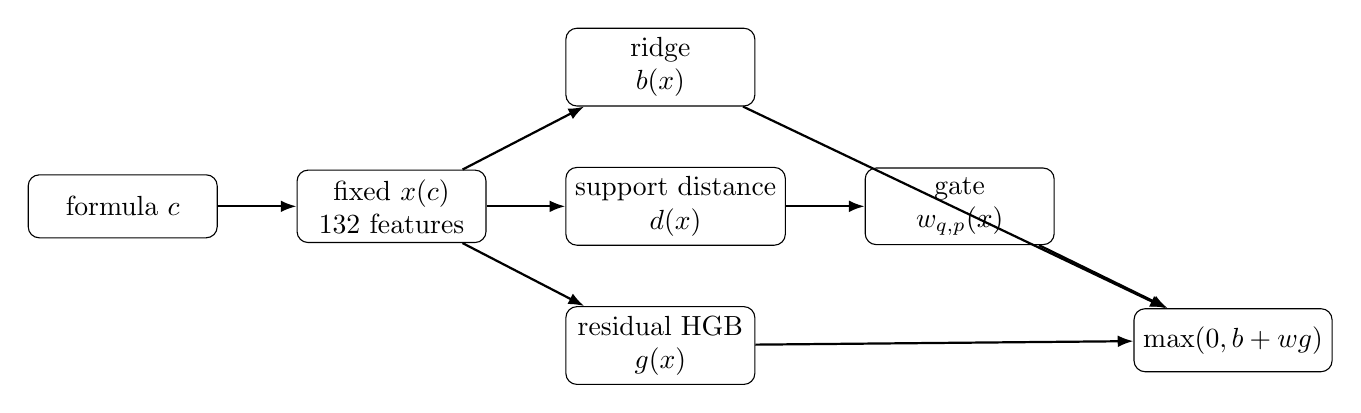
\begin{tikzpicture}[
 node distance=8mm and 10mm,
 box/.style={draw,rounded corners,align=center,minimum height=8mm,minimum width=24mm},
 arrow/.style={-{Latex[length=2mm]},thick}
]
\node[box] (formula) {formula $c$};
\node[box,right=of formula] (feat) {fixed $x(c)$\\132 features};
\node[box,above right=of feat] (ridge) {ridge\\$b(x)$};
\node[box,right=of feat] (distance) {support distance\\$d(x)$};
\node[box,below right=of feat] (residual) {residual HGB\\$g(x)$};
\node[box,right=of distance] (gate) {gate\\$w_{q,p}(x)$};
\node[box,below right=of gate] (output) {$\max(0,b+wg)$};
\draw[arrow] (formula)--(feat);
\draw[arrow] (feat)--(ridge);
\draw[arrow] (feat)--(distance);
\draw[arrow] (feat)--(residual);
\draw[arrow] (distance)--(gate);
\draw[arrow] (ridge)--(output);
\draw[arrow] (residual)--(output);
\draw[arrow] (gate)--(output);
\end{tikzpicture}
}
\caption{The gate acts only on the nonlinear residual. The ungated control fixes
$w=1$ while retaining the same fitted ridge and residual models.}
\label{fig:architecture}
\end{figure}

\subsection{Complexity and failure behavior}
For $n$ rows, $d=132$ features, and $T$ boosting iterations, ridge fitting is
bounded by the library solver, histogram boosting is approximately
$O(Tnd)$ aside from tree overhead, and brute-force support fitting/querying is
$O(n^2d)$/$O(nmd)$ for $m$ queries at this dataset scale. Any non-finite
feature, distance, or prediction is fatal. Model outputs are clipped only at the
physical lower bound zero; no upper target bound is imposed.

\begin{algorithm}[t]
\caption{Frozen development selection}
\begin{algorithmic}[1]
\For{$E\in\{\mathrm{Cu},\mathrm{Ag},\mathrm{B}\}$}
  \State exclude every composition containing $E$ from training
  \State fit ridge and one residual learner
  \For{$q\in\{0.80,0.90,0.95,0.99\}$ and $p\in\{1,2\}$}
    \State evaluate $h_{q,p}$ on all compositions containing $E$
  \EndFor
  \State evaluate median, ridge, direct HGB, and ungated residual controls
\EndFor
\State select the minimum macro-MAE gate
\State for candidates within 0.002 eV, choose lower $p$, then higher $q$
\State emit a hash-verified freeze candidate; do not open confirmation
\end{algorithmic}
\end{algorithm}

\section{Experimental Methodology}
\subsection{Dataset and integrity}
We use Matbench v0.1 \texttt{matbench\_expt\_gap}, 4,604 compositions with
experimental band gaps from 0.0 to 11.7 eV. The compressed artifact is accepted
only at SHA-256
{\footnotesize\ttfamily 783e7d1461eb83b00b2f2942da4b95fda5e58a0d1ae26b581c24cf8a82ca75b2}.
Local scale/order canonicalization yields 4,601 unique compositions. The
official five-fold split is regenerated with the declared Matbench seed and
must match a separately retained canonical digest. Official folds contain
known canonical overlap in folds 0--3 and are not treated as OOD evidence.

\subsection{Controls and endpoints}
Controls are a training-target median, ridge, a direct HGB model, and the
compute-matched ungated residual. Development sees Cu, Ag, and B only. The
protected confirmatory elements are Li, Zn, Ga, Se, and Te. Confirmation is
supported only if $\bar\Delta>0.01$ eV, at least four of five element effects
are positive, and official pooled MAE is no more than 0.02 eV worse than the
ungated control. We report per-element MAE, RMSE, median absolute error, bias,
gate statistics, runtime, peak RSS, and pageouts.

\subsection{Uncertainty and statistics}
For each official fold, a separate 80/20 split of the outer-training rows forms
proper training and calibration sets. If calibration absolute residuals sorted
as $s_{(1)}\le\cdots\le s_{(n_c)}$, the 90\% split-conformal radius is
\begin{equation}
 q_{0.9}=s_{(k)},\qquad k=\min\{n_c,\lceil(n_c+1)0.9\rceil\}.
\end{equation}
Intervals are $[\max(0,\hat y-q_{0.9}),\hat y+q_{0.9}]$. We report observed
coverage, mean width, and interval score. These are marginal IID diagnostics.

The five element improvements are reported individually, with a 10,000-resample
bootstrap over elements and an exact one-sided sign-permutation statistic. The
small, overlapping scenario set precludes strong asymptotic claims; the
practical-effect and sign-count rule is primary.

\subsection{Resource, provenance, and stopping rules}
Each run must begin and remain below 512 MiB peak process RSS, with no increase
in macOS \texttt{Pageouts} or Linux \texttt{pswpout}. Every phase is checked.
A refusal writes a failure trace, resource observations, receipt, and a
SHA-256 manifest, then stops without weakening the gate. Run IDs are immutable.
The development budget ends after eight gates; protected confirmation runs once
under a separately frozen protocol.

\section{Implementation Verification}
The package exposes \texttt{prepare}, \texttt{preflight}, \texttt{develop},
\texttt{confirm}, and \texttt{verify}. Formula tests cover nested groups,
fractional stoichiometry, scaling invariance, and malformed input. Mathematical
tests hand-check regression and interval metrics. Split tests regenerate all
fold sizes, prove train/test disjointness and completeness, and match the
canonical split digest. Model tests show that in-support gates equal one,
far-out gates decay, and the mechanism-off prediction equals $b+g$. Manifest
tests substitute and add files to ensure verification fails closed.

The isolated Python 3.12 environment resolves 29 packages. Twelve tests pass;
the source distribution and wheel build successfully. This establishes
software behavior, not scientific performance.

\section{Execution Results}
Table~\ref{tab:execution} is the complete outcome-bearing record at this stage.
No fold, element scenario, predictive metric, or interval result exists.

\begin{table}[h]
\centering
\caption{Execution receipts before hosted development.}
\label{tab:execution}
\begin{tabularx}{\linewidth}{>{\raggedright\arraybackslash}p{0.25\linewidth}>{\raggedright\arraybackslash}p{0.18\linewidth}>{\raggedright\arraybackslash}X}
\toprule
Run or gate & Status & Verified observation \\
\midrule
Dataset preparation & PASS & 4,604 rows; source and official-split digests match \\
Software suite & PASS & 12 tests; package and wheel build \\
Local preflight & ADMITTED & 124.5 MiB peak RSS; pageout delta 0 \\
Local development v1-r1 & FAILED & retained after features; 129.3 MiB peak RSS; pageouts +8 \\
Hosted development & NOT EXECUTED & explicit source-export authorization required \\
Confirmatory study & NOT AUTHORIZED & no development freeze candidate exists \\
\bottomrule
\end{tabularx}
\end{table}

The local failure occurred before fitting any model. It cannot support or refute
the mechanism, and it supplies no basis for selecting a gate. The evidence does
support a narrower engineering conclusion: the feature path fits well below
the RSS ceiling, but this macOS host does not satisfy the no-rising-pageout
condition even for the bounded preparation phase. This reproduces the
predecessor's resource limitation rather than curing it by relaxing the rule.

\section{Failure Analysis and Threats to Validity}
\paragraph{Representation.} Atomic-number, period, and group moments are coarse;
distance in this space is neither chemical equivalence nor an error probability.
\paragraph{Identifiability.} Composition-only inputs conflate polymorphs and
experimental contexts, imposing irreducible ambiguity.
\paragraph{Selection.} Eight gate candidates may overfit three development
elements; confirmation is therefore separated and immutable.
\paragraph{Dependence.} Element test sets overlap, so five effects are not five
independent samples from a well-defined population.
\paragraph{Benchmark leakage.} Canonical duplicates across official folds can
optimistically bias IID compatibility metrics.
\paragraph{Baselines.} The controls isolate the gate but do not establish
state-of-the-art performance against every deep composition model. A positive
mechanism result would be an ablation result, not an overall leaderboard claim.
\paragraph{Conformal scope.} Marginal coverage relies on exchangeability and is
not promised under the protected element shift.

\section{Discussion}
The study design makes a narrow improvement hard to fake. Capacity and training
compute are matched because the gate operates after the same ridge and residual
models are fitted. IID and shifted endpoints are separated. The development
grid and tie-break are fixed. A valid negative outcome would show that support
distance does not reliably identify harmful residual corrections in this
representation; a mixed outcome would motivate studying which chemical regimes
make the linear fallback safer, but only in a separately versioned successor.

Even a supported result would not make \method{} a materials-discovery engine.
It would establish that one conservative intervention improved one
composition-only extrapolation protocol while preserving one public benchmark
within tolerance. Candidate stability, synthesis, novelty, and utility would
remain untested.

\section{Conclusion}
We have specified and implemented a fully matched test of support-gated residual
learning for experimental band gaps. The data, splits, model, development
budget, protected elements, statistical rules, and failure behavior are frozen.
Software and data-integrity gates pass, while the first numerical attempt was
resource-refused before model fitting. Consequently, the scientifically correct
current disposition is \texttt{NOT\_EVALUATED}, not a favorable result. Hosted
development, confirmatory freezing, and one protected execution are the exact
remaining steps before the central question becomes answerable.

\section*{Reproducibility Statement}
The repository contains the canonical research state, machine-readable protocol,
dataset and model cards, pinned lockfile, exact source and split digests, test
suite, package build configuration, hosted runner, failed local receipt, and
artifact verifier. A hosted run must emit its environment, source revision,
resource trace, raw per-condition metrics, model checkpoints, receipt, and file
manifest. Numerical manuscript text may be regenerated only from a successful,
manifest-valid confirmatory bundle.

\bibliographystyle{plainnat}
\bibliography{references}

\appendix
\section{Chronological Forward, Training, and Inference Processes}
At training time the parser produces normalized fractions, the featurizer emits
132 finite values, ridge fits the target, HGB fits ridge residuals, the support
standardizer and neighbour index fit training descriptors, and the training
leave-one-out distances determine $\tau_q$. At inference the same parser and
feature order are used; ridge, residual, nearest distance, gate, and non-negative
projection are applied in that order. No test label enters any transformation.

\section{Claim-Evidence Matrix}
\begin{tabularx}{\linewidth}{>{\raggedright\arraybackslash}p{0.34\linewidth}>{\raggedright\arraybackslash}p{0.33\linewidth}>{\raggedright\arraybackslash}X}
\toprule
Claim & Required artifact & Current state \\
\midrule
Input and folds are pinned & dataset receipt and split digest & supported \\
Implementation follows equations & tests and source & supported as software \\
Gate improves element exclusion & protected element metrics & not evaluated \\
Gate preserves official MAE & official OOF prediction table & not evaluated \\
90\% intervals calibrate & fold interval metrics & not evaluated \\
Method discovers materials & structural/experimental evidence & prohibited \\
\bottomrule
\end{tabularx}

\section{Exact Reproduction Commands}
\begin{verbatim}
UV_CACHE_DIR=/tmp/sparking-uv-cache uv sync --extra dev --locked
UV_CACHE_DIR=/tmp/sparking-uv-cache uv run sparking prepare
UV_CACHE_DIR=/tmp/sparking-uv-cache uv run pytest -q
UV_CACHE_DIR=/tmp/sparking-uv-cache uv run sparking preflight
UV_CACHE_DIR=/tmp/sparking-uv-cache uv run sparking develop \
  --run-id development-v1
UV_CACHE_DIR=/tmp/sparking-uv-cache uv run sparking verify \
  --run-id development-v1
\end{verbatim}

\end{document}

